

\section{Abstract}
Rossby waves are a way to conceptualize large scale, time-dependent motion in the atmosphere and ocean. Analytically we expect Rossby waves to travel westwards, and this was tested numerically with different time-stepping methods for a periodic and finite domain. \\

The numerical results show that Rossby waves travel westwards. For the finite domain the Rossby wave hits the wall and is reflected backwards to the east. This results in some resonance for the finite case. For the periodic case only regular sinusoidal shaped waves of constant amplitude was observed.




\section{Introduction}
In this project I will study Rossby waves. Rossby waves are a way to conceptualize large scale, time-dependent motion in the atmosphere and ocean. These waves typically have scales of hundreds to thousands of kilometers. Two examples of phenomenon that we try to understand with Rossby waves is the meandering of the atmospheric Jet Stream, and the adjustment of the ocean to changes in wind forcing, also called geostrophic adjustment.\cite{geofludyn}

Rossby waves exist because of the Coriolis acceleration, which acts perpendicular to the velocity of a fluid parcel. In the Northern Hemisphere we have positive Coriolis acceleration, and in the Southern Hemisphere we have negative Coriolis. The Coriolis acceleration varies with latitude, strengthens towards the poles and weakens towards the equator. This is also why Rossby waves are treated a bit differently around the equator, and most of the time examined in mid- or high- latitudes. \cite{rossby}

Around the equator we usually apply the equatorial beta plane approximation ($f=\beta y$, where $\beta$ is the variation of Coriolis in the y-direction(north-south) given by $\beta = df/dy$), where we may study equatorial Kelvin waves, which are lightning bolts compared to Rossby waves. Without a mean flow, equatorial Rossby waves (slow waves propagating with speeds on order of cm/s) are observed to travel west and Kelvin waves travel east (propagation speeds on order of m/s) around the equator.\cite{equator}\\


The variation in Coriolis acceleration with latitude causes fluid parcels to change their spin, in context of a continuum called the vorticity \cite{vorticity}, as they move to different latitudes.\\

Introducing short hand notations for derivatives in as shown below:\\

$\partial_t = \frac{\partial}{\partial t}$\\

$\partial_x = \frac{\partial}{\partial x}$\\

$\partial_{xx} = \frac{\partial^2}{\partial x^2}$\\

The vorticity equation is then given as:\\ 

\begin{equation}
\partial_t\zeta + \beta\partial_x\psi = 0
\end{equation}\\

Where $\zeta$ is the vorticity, $\beta$ comes from the $\beta$-plane approximation explained below and $\psi$ is the streamfunction determining the velocities:\\

\begin{equation}
u = -\partial_y\psi  \\\   ,  \\\  v = \partial_x\psi
\end{equation}\\

Where u is the east-west velocity and v is the north-south velocity.\\

Vorticity is defined as the curl, and the horizontal Laplacian of the streamfunction:\\

\begin{equation}
\zeta = \partial_xv - \partial_yu = \nabla^2_H\psi
\end{equation}\\

The Coriolis parameter is defined by:\\

\begin{equation}
f = 2\Omega sin(\theta)
\end{equation}\\

where $\theta$ is the latitude and $\Omega$ is the rotation rate of the earth, $\Omega = 2\pi/day$. As hinted at before, we often approximate f as a linear function centered on a latitude $\theta_0$:\\

\begin{equation}
f\approx f_0 + \beta y
\end{equation}\\

where $f_0 = 2\Omega sin(\theta_0)$, $\beta = 2\Omega cos(\theta_0)/R_e$ and $y = R_e(\theta - \theta_0)$, if $R_e$ is the Earth's radius. This linear representation is called the $\beta$-plane approximation and is the $\beta$ term in equation (1). Using the definition of vorticity we can rewrite the vorticity equation (1) in terms of only one variable, the streamfunction:\\

\begin{equation}
\partial_t\nabla^2_H\psi + \beta\partial_x\psi = 0
\end{equation}\\

This is the barotropic Rossby wave equation, barotropic meaning that the density variations are only dependent on the change in pressure.\\

We will examine solutions of the vorticity equation in a periodic and closed domain, both analytically and numerically. For the periodic case we can consider a re-entrant domain, like going around the Earth's atmosphere. For a closed domain we can think of continents acting as walls bounding the ocean.

 



\section{Methods}
\subsection{Analytical solutions}
My calculations are mainly based on the lecture notes from geophysical fluid dynamics: \cite{geofludyn}\\

\subsubsection{Solution to the Rossby equation in a periodic domain}
Consider the vorticity equation from (6) in one dimension. Assuming the periodic domain in x = [0,L] I can propose a wave solution on the form:\\

\begin{equation}
\psi = Acos(\frac{2n\pi x}{L}-\omega t)
\end{equation}\\

, where n is an integer, $\omega$ is the wave frequency and A is the amplitude.\\

I need to show that the solution on the two boundaries are the same, satisfying periodic domain, and then solve for $\omega$ to find the dispersion relation. Using the proposed wave solution in (7) I have the following:\\

\begin{equation}
\begin{gathered}
\zeta = \partial_xv = \partial_{xx}\psi\\
\partial_x\psi = -A\frac{2n\pi}{L}sin(\frac{2n\pi x}{L}-\omega t)\\
\zeta = \partial_{xx}\psi = -A(\frac{2n\pi}{L})^2cos(\frac{2n\pi x}{L}-\omega t)\\
\zeta(x=0,t) = -A(\frac{2n\pi}{L})^2cos(-\omega t)\\
\zeta(x=L,t) = -A(\frac{2n\pi}{L})^2cos(\frac{2n\pi L}{L}-\omega t) = -A(\frac{2n\pi}{L})^2cos(2n\pi-\omega t) = -A(\frac{2n\pi}{L})^2cos(-\omega t)\\
\end{gathered}
\end{equation}

Equation 8 shows that periodic boundary conditions are ok. Inserting $\zeta$ into equation (6) yields:\\

\begin{equation}
\begin{gathered}
\partial_t\nabla^2_H\psi + \beta\partial_x\psi = \partial_t\zeta + \beta\partial_x\psi =\\
-A(\frac{2n\pi}{L})^2\omega \sin(\frac{2n\pi x}{L}-\omega t) - \beta A\frac{2n\pi}{L}\sin(\frac{2n\pi x}{L}-\omega t)\\
\implies A\frac{2n\pi}{L}(\frac{2n\pi \omega}{L}+\beta)\sin(\frac{2n\pi x}{L}-\omega t) = 0\\
\implies \omega = -\frac{\beta L}{2\pi n}
\end{gathered}
\end{equation}

This is the dispersion relation of the wave. The phase speed is the speed at which Rossby waves move. Consider the phase of the wave as:\\

$\theta = \frac{n\pi x}{L}-\omega t$\\

If we choose $\theta = 2\pi$ we get $\psi = Acos(2\pi) = A$, which means that we have a high pressure point with amplitude A. Solving for x we can find how this point moves, and taking the time derivative of that expression gives us an expression for the phase speed:\\

$x = \frac{\theta L}{2n\pi} + \frac{\omega tL}{2n\pi}$\\

$c = \frac{dx}{dt} = \frac{\omega L}{2n\pi}$\\

Inserting my expression for $\omega$ I get the Rossby phase speed in the x direction:\\

$c_x = \frac{\omega L}{2n\pi} = -\beta(\frac{L}{2n\pi})^2$\\

Thus, I find that the Rossby wave is moving westwards.\\

\subsubsection{Solution to the Rossby equation with solid boundaries} 

In the ocean it's more appropriate to apply boundary conditions of no flow at the two end points. This can be enforced with Dirichlet conditions: $\psi = 0$ at $x=0$ and $x=L$. Proposing a wave solution of the form:\\

\begin{equation}
\psi = A(x)cos(kx-\omega t)
\end{equation}\\

, where A(x) indicates that the amplitude has a structure which must be solved for the boundary conditions. Inserting the wave solution above into equation (6) I get the following:\\

\begin{equation}
\begin{gathered}
\psi(x=0,t) = \psi(x=L,t)=0\\
\psi(x,t)=A(x)cos(kx-\omega t)\\
\partial_x\psi = A'(x)cos(kx-\omega t) - A(x)ksin(kx-\omega t)\\
\zeta = \partial_{xx}\psi = A''(x)cos(kx-\omega t)-A'(x)ksin(kx-\omega t) - A'(x)ksin(kx-\omega t) - A(x)k^2cos(kx-\omega t) =\\
(A''(x)-A(x)k^2)cos(kx-\omega t)-2A'(x)ksin(kx-\omega t)\\
\implies \partial_t\zeta + \beta\partial_x\psi =\\
(A''(x)-A(x)k^2)\omega sin(kx-\omega t)+2A'(x)k\omega cos(kx-\omega t) + \beta(A'(x)cos(kx-\omega t) - A(x)ksin(kx-\omega t))\\
\implies ((A''(x)-A(x)k^2)\omega - \beta A(x)k)sin(kx-\omega t) + A'(x)(2k\omega + \beta)cos(kx-\omega t) = 0
\end{gathered}
\end{equation}\\

This holds if:\\

$(A''(x)-A(x)k^2)\omega - \beta A(x)k = 0$\\

and solving for $\omega$ I find an initial expression for the dispersion relation. \\

$2k\omega + \beta = 0$\\
$\implies \omega = \frac{-\beta}{2k}$\\

and

$c_x = \frac{\omega}{k} = \frac{-\beta}{2k^2}$\\


Solving for the structure:\\

\begin{equation}
\begin{gathered}
A''(x) - A(x)(k^2+\frac{\beta k}{\omega} = 0\\
r^2-(k^2+\frac{\beta k}{\omega})=0\\
r = \pm k\sqrt{1+\frac{\beta}{k\omega}}\\
= \pm k\sqrt{1-\frac{\beta}{k\beta/2k}} = \pm k\sqrt{1-2} = \pm ik\\
\implies A(x) = C\cos(kx) + D\sin(kx)
\end{gathered}
\end{equation}\\

Need to satisfy Dirichlet conditions:\\

\begin{equation}
\begin{gathered}
\psi(x=0,t) = A(0)\cos(-\omega t) = 0\\
\implies C + D\sin(0) = 0
\implies C = 0\\
\psi(x=L,t) = A(L)\cos(kL-\omega t) = 0\\
\implies A(L) = D\sin(kL) = 0\\
\implies kL = n\pi\\
\implies k_n = \frac{n\pi}{L}\\
\end{gathered}
\end{equation}\\

I find that the allowed frequencies given by the dispersion relation becomes:\\

$\omega_n = \frac{-\beta L}{2\pi n}$\\

and the Rossby phase speed:\\

$c_x = \frac{\omega_n}{k_n} = \frac{\beta}{2}(\frac{L}{n\pi})^2$\\

The full wave solution becomes:\\

\begin{equation}
\psi(x,t) = D\sin(\frac{n\pi x}{L})\cos(\frac{n\pi x}{L}+\frac{\beta Lt}{2\pi n})
\end{equation}

, where D must be determined from the initial conditions for a specific problem.




\subsection{Method for solving the barotropic Rossby wave equation numerically}
A numerical solution to equation (6), involves two steps. If we know the velocity or streamfunction initially, we can advance the vorticity in time to a new time. Then the streamfunction at the new time is found by inverting equation (3). This process is repeated to find a complete numerical solution.\\

Since the vorticity does not vary with change in y-direction for the one dimensional case I have:\\

\begin{equation}
\zeta = \partial_{xx}\psi
\end{equation} 

This is a specification of equation (3), which is solved as the Poisson equation, the same way as used in project 1. We have the same form:\\

$u''(x) = f(x)$ , the Poisson structure is recognized as:\\

$\partial_{xx} \psi = \zeta$\\

which, for the rigid boundary conditions can be solved the exact same way: 

To discretize the equations, we assume a grid of equally-spaced
points:

\begin{equation}
x_j = j\Delta x
\end{equation}
where $\Delta x$ is the grid spacing. We discretize time in a similar way:

\begin{equation}
t^n = n\Delta t
\end{equation}
where $\Delta t$ is the time step. Thus $t^0=0$, $t^1=\Delta t$, and so on.\\

We then approximate the derivatives by finite differences. For
the spatial derivatives, we use centered-differences:

\begin{align}
	\partial_x\psi &\approx \frac{\psi_{j+1}^{n} - \psi_{j-1}^{n}}{2\Delta x}, \\
	\partial_{xx}\psi &\approx \frac{\psi_{j+1}^{n} - 2\psi_{j}^{n} + \psi_{j-1}^{n}}{\Delta x^2},
\end{align}

Thus the discretized 1D Poisson equation becomes a set of algebraic equations:\\


\begin{align}
\implies \psi_{j+1}^{n} - 2\psi_{j}^{n} + \psi_{j-1}^{n} = \zeta_j^n {\Delta x^2}
\end{align}

, where j is the space step j = 1,2,...,$j_{max}$\\

For periodic boundary conditions it's much more difficult to satisfy the boundary conditions. The boundary at x=0 we must be carefully handled with an extra imaginary point $x_{-1}$, since we have that the last step should be the first step for the next cycle. For j = 0 I get:\\

\begin{align}
\psi_{1}^{n} - 2\psi_{0}^{n} + \psi_{-1}^{n} = \zeta_0^n {\Delta x^2}
\end{align}\\

, where $\psi_{-1}^{n}$ is the problem term. To solve it I utilize equation (18), by saying that\\ 

\begin{align}
\partial_x \psi_{0}^{n} = \frac{\psi_{1}^{n} - \psi_{-1}^{n}}{2\Delta x}
\end{align}\\
 
Rearranging and solving the equation in regards to 
$\psi_{-1}^{n}$ I get:\\

\begin{align}
\psi_{-1}^{n} = \psi_{1}^{n} - 2\Delta x \partial_x \psi_{0}^{n}
\end{align}\\

Substituting this expression into the previous equation (21) I get:\\

\begin{align}
\psi_{1}^{n} - 2\psi_{0}^{n} + \psi_{1}^{n} - 2\Delta x \partial_x \psi_{0}^{n} = \zeta_0^n {\Delta x^2}
\end{align}

Rearranging again I get the result of the boundary condition:\\

\begin{align}
\psi_{1}^{n} - \psi_{0}^{n}  = \frac{\zeta_0^n {\Delta x^2} + 2\Delta x \partial_x \psi_{0}^{n}}{2}
\end{align}\\

Now we can introduce the vector $\mathbf{F}$, as done in equation 5 of \cite{poisson}. The elements of $\mathbf{F}$ are $F_j$ defined by:\\

\begin{equation}
\begin{gathered}
F_0 = \frac{\zeta_0^n {\Delta x^2}}{2} + \Delta x \partial_x\psi_0\\
F_{j_{max}} = \Delta x^2 \zeta_{j_{max}} - \psi_0\\
F_j = \Delta x^2 \zeta_j
\end{gathered}
\end{equation}

, where j = 1, 2, ..., $j_{max}-1$\\

I obtain the following matrix equation:\\

\[
\begin{bmatrix}
       -1& 1& 0 &\dots   & \dots &0 \\
       1 & -2 & 1 &0 &\dots &\dots \\
       0&1 &-2 & 1 & 0 & \dots \\
       & \dots   & \dots &\dots   &\dots & \dots \\
       0&\dots   &  &1 &-2& 1 \\
       0&\dots    &  & 0  &1 & -1 \\
\end{bmatrix}
\begin{bmatrix}
	\psi_0 \\
	\psi_1 \\
	\psi_2 \\
	\vdots \\
	\psi_{j_{max}-1} \\
	\psi_{j_{max}} \\                      
\end{bmatrix} = 
\Delta x^2
\begin{bmatrix}
	\zeta_0 \\
	\zeta_1 \\
	\zeta_3 \\
	\vdots \\
	\zeta_{j_{max}-1} \\
	\zeta_{j_{max}} \\                      
\end{bmatrix}
\]\\

This tridiagonal matrix is then solved numerically with the Thomas algorithm as prescribed in \cite{trisolve} or chapter 6.4 in \cite{lecturenote}.\\

Equation (6) is a prognostic equation, which will be solved numerically by using a time-stepping method.


For the time stepping, we will test two methods. One involves a
forward difference:

\begin{equation}
  \label{eq:Rossby3}
  \partial_t\psi \approx \frac{\psi_{j}^{n+1} - \psi_{j}^{n}}{\Delta t} ,
\end{equation}

while the second involves a centered difference:

\begin{align}
  \label{eq:Rossby4}
	\partial_t\psi &\approx \frac{\psi_{j}^{n+1} - \psi_{j}^{n-1}}{2\Delta t}.
\end{align}\\

The forward method is rearranged to be solved using the following algorithm\\

\begin{align}
\zeta_j^{n+1} = \Delta t(\frac{\psi_{j+1}^n-\psi_{0}^n}{\Delta x})+\zeta_j^{n}
\end{align}\\

and the central method is rearranged to:\\

\begin{align}
\zeta_j^{n+1} = 2\Delta t(\frac{\psi_{j+1}^n-\psi_{j-1}^n}{2\Delta x})+\zeta_j^{n-1}
\end{align}\\


 






\newpage
\section{Implementation}
For all programs, see:\\
$\href{https://github.com/larsjbro/FYS4150/tree/master/project_4/source}{https://github.com/larsjbro/FYS4150/tree/master/project_5/source}$


\subsection{Tridiagonal matrix solver}
The Thomas method is implemented to find an expression for the vorticity. This method is implemented in the functions

\begin{verbatim}
tridiagonal_solve_specific
\end{verbatim}

is used for solving the finite domain

and 

\begin{verbatim}
tridiagonal_solve
\end{verbatim}

is used to solve for the periodic domain.

The result from the solver is then inserted into the Rossby wave equation and solved with time stepping methods.

\subsection{Rossby wave solution for finite and periodic domain}
A solver for the barotropic Rossby wave equation for finite and perodic domain is implemented with the functions

\begin{verbatim}
solve_rossby_with_walls
\end{verbatim}

and

\begin{verbatim}
solve_rossby_periodic
\end{verbatim}

respectively.

%*Code/Implementations/test: Readability of code, implementation, testing and discussion of benchmarks. Total number of possible points 20*

 

\section{Results}
%*Analysis: of results and the effectiveness of their selection and presentation. Are the results well understood and discussed? Total number of possible points: 20*

\subsection{Agreement between analytical and numerical simulations}

Theoretically we expect the Rossby wave to travel westwards barring a strong mean flow to the east. From figure 1 and 2 I see that this case is confirmed, as I can see the wave moving westwards with increasing time. I can also see that the waves are interfering as the amplitude of the waves are changed with time for the finite domain!

\subsubsection{Finite domain}
Figure 1 and 2 shows the Rossby wave propagation going westwards and also showing some change in amplitude due to the finite boundaries resulting in reflection of waves. 


\FloatBarrier
\begin{figure}[!ht]
\centering
\FloatBarrier
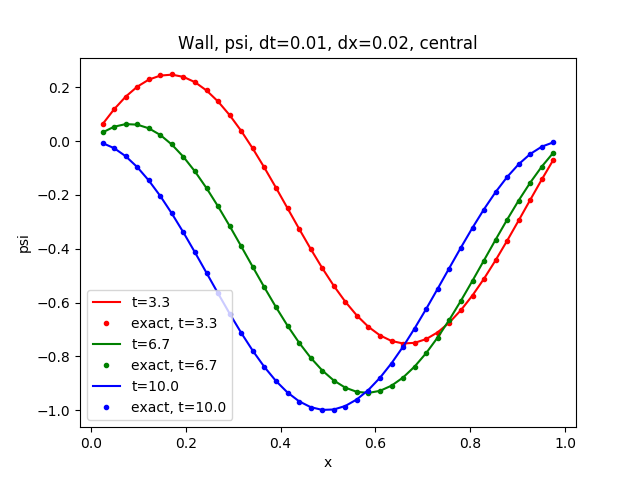
\includegraphics[width=0.70\textwidth]{task_5c_psi_Wall_central1000.png}

\caption{Plot of streamfunction for finite domain with central method, for three different times}
\label{fig:Earth_orbit_sun_Forward_Euler_k_2}
\end{figure}
\FloatBarrier


\FloatBarrier
\begin{figure}[!ht]
\centering
\FloatBarrier
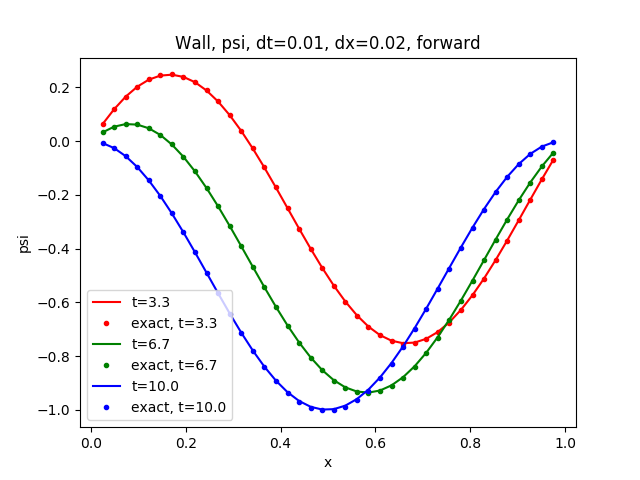
\includegraphics[width=0.70\textwidth]{task_5c_psi_Wall_forward1000.png}

\caption{Plot of streamfunction for finite domain with forward stepping method, for three different times.}
\label{fig:Earth_orbit_sun_Forward_Euler_k_2}
\end{figure}
\FloatBarrier

\subsubsection{Periodic domain}
Figure 3 and 4 show that also the periodic waves travel westwards but are are not distorted in their shape, which is because there is no reflection at a wall.


\FloatBarrier
\begin{figure}[!ht]
\centering
\FloatBarrier
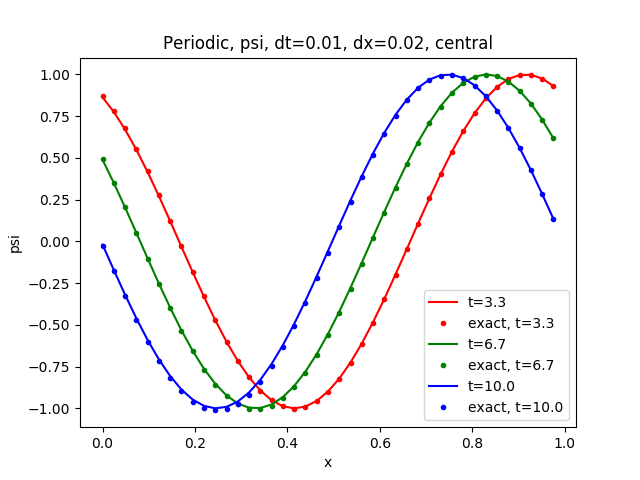
\includegraphics[width=0.70\textwidth]{task_5c_psi_Periodic_central1000.png}

\caption{Plot of streamfunction for periodic domain with central stepping method, for three different times.}
\label{fig:Earth_orbit_sun_Forward_Euler_k_2}
\end{figure}
\FloatBarrier


\FloatBarrier
\begin{figure}[!ht]
\centering
\FloatBarrier
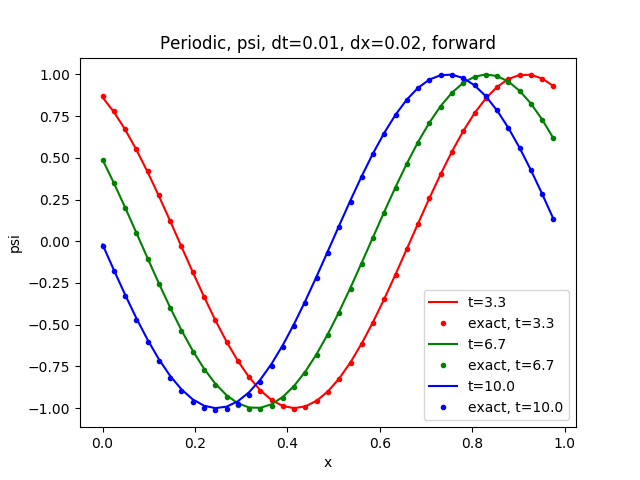
\includegraphics[width=0.70\textwidth]{task_5c_psi_Periodic_forward1000.png}

\caption{Plot of streamfunction for periodic domain with forward stepping method, for three different times.}
\label{fig:Earth_orbit_sun_Forward_Euler_k_2}
\end{figure}
\FloatBarrier









\section{Conclusion}
Barotropic Rossby waves travel in the western direction, but the numerical solution to the problem is quite difficult. Especially for the case of a periodic domain, when the boundary conditions introduced a stepping problem. 

I find that the central method was slightly better as a numerical method. I also find that the Rossby waves travel westwards for both the periodic and the finite domain. In the finite domain I can see that the amplitude of the wave is distorted which is a sign that there is reflection of waves at the walls resulting in resonance.


%*Conclusions, discussions and critical comments: on what was learned about the method used and on the results obtained. Possible directions and future improvements? Total number of possible points: 10*




\begin{thebibliography}{99}
\bibitem{lecturenote}$\href{https://github.com/CompPhysics/ComputationalPhysics/blob/gh-pages/doc/Lectures/lectures2015.pdf}{https://github.com/CompPhysics/ComputationalPhysics/blob/gh-pages/doc/Lectures/lectures2015.pdf}$, November 19 2017\\
\bibitem{equator}$\href{https://en.wikipedia.org/wiki/Equatorial\_wave}{https://en.wikipedia.org/wiki/Equatorial\_wave}$
\bibitem{geofludyn}$\href{http://folk.uio.no/josepl/papers/dynbook7.pdf}{http://folk.uio.no/josepl/papers/dynbook7.pdf}$
\bibitem{rossby}$\href{https://en.wikipedia.org/wiki/Rossby\_wave}{https://en.wikipedia.org/wiki/Rossby\_wave}$
\bibitem{poisson}$\href{http://file.scirp.org/pdf/JEMAA_2014092510103331.pdf}{http://file.scirp.org/pdf/JEMAA_2014092510103331.pdf}$
\bibitem{vorticity}$\href{https://en.wikipedia.org/wiki/Vorticity}{https://en.wikipedia.org/wiki/Vorticity}$
\bibitem{trisolve}$\href{https://www.cfd-online.com/Wiki/Tridiagonal\_matrix\_algorithm\_-\_TDMA\_(Thomas\_algorithm)}{https://www.cfd-online.com/Wiki/Tridiagonal\_matrix\_algorithm\_-\_TDMA\_(Thomas\_algorithm)}$
\end{thebibliography}




%\FloatBarrier
%\begin{figure}[!ht]
%\centering
%\FloatBarrier
%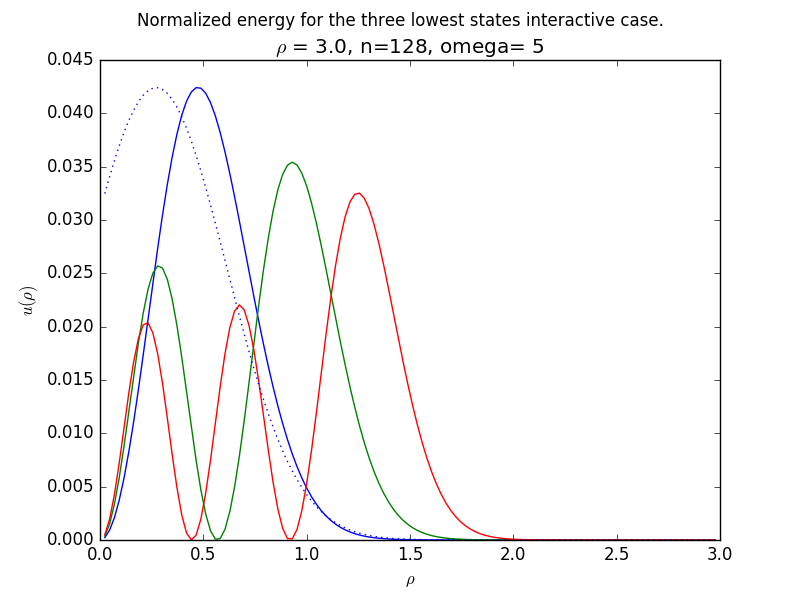
\includegraphics[width=0.45\textwidth]{eigenvector_rho29n128omega500.png}
%
%\caption{Normalized energy for the three lowest eigenvalues for repulsive Coulomb interaction with n=128 and $\omega_r$=5}
%\label{fig:Eigenvalue_states_n_320_omega_500}
%\end{figure}
%\FloatBarrier


